\section{Optical Instruments} \index{Optical instruments}

\begin{multicols}{2}


\subsection{Simple Microscope} \index{Microscope}

\begin{center}
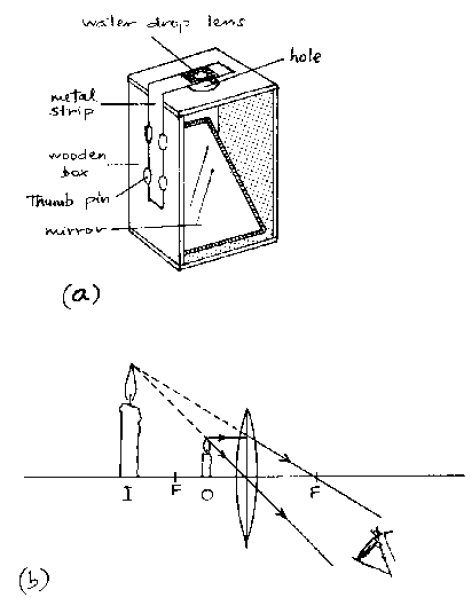
\includegraphics[width=0.49\textwidth]{./img/source/simple-microscope.png}
\end{center}

\begin{description*}
%\item[Subtopic:]{}
\item[Materials:]{Mirror, thumb pins, wooden box, metal strip, knife}
\item[Setup:]{Construct the simple microscope according to the figure above.}
\item[Procedure:]{Adjust the mirror so that sun rays are reflected to the hole below the lens. Place a transparent object (e.g. wing of a fly) on the hole and adjust the metal strip so that the water drop lens has less distance from the object than its focal length, as shown in the ray diagram.}
%\item[Hazards:]{}
%\item[Questions:]{}
%\item[Observations:]{}
\item[Theory:]{The lens acts as a magnifying glass. When the object distance decreases, the magnification increases}
%\item[Applications:]{}
\item[Notes:]{For more ideas on locally available microscopes, see the section on \nameref{cha:microscopy} (p.~\pageref{cha:microscopy}).}
\end{description*}

\vfill
\columnbreak

%\subsection{Magnification}
%
%\begin{center}
%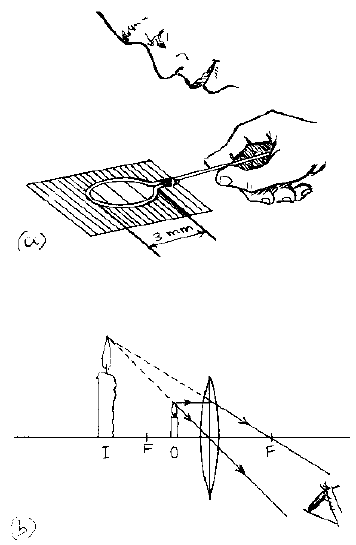
\includegraphics[width=0.45\textwidth]{./img/source/magnification.png}
%\end{center}
%
%\begin{description*}
%%\item[Subtopic:]{}
%\item[Materials:]{Paper clip, pen, water bottle, water}
%\item[Setup:]{Make a loop using paper clip wire and wind around a pen to construct a magnifying glass.}
%\item[Procedure:]{Dip the loop in water and use the magnifying glass to observe small objects or letters in a book. Alternatively, fill a water bottle and hold it over the object/letters.}
%%\item[Hazards:]{}
%%\item[Questions:]{}
%%\item[Observations:]{}
%\item[Theory:]{The water drop and water bottle act as convex lenses. According to the ray diagram shown, the image is larger than the object. The image is also virtual and the object distance is less than the focal length.}
%\item[Applications:]{Magnifying glass, microscopes, telescopes, etc.}
%%\item[Notes:]{}
%\end{description*}

\subsection{Human Eye}

\begin{center}
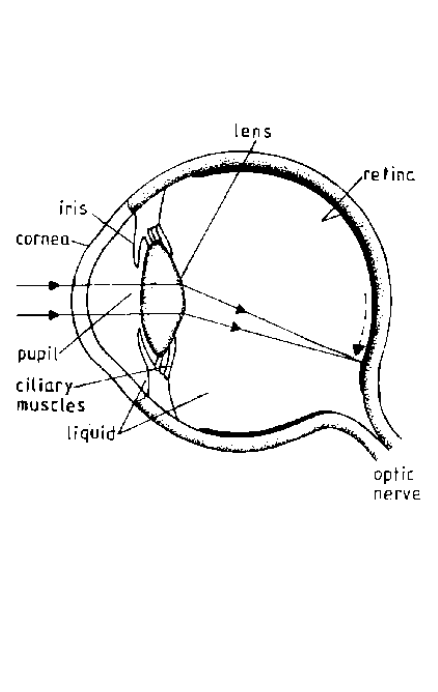
\includegraphics[width=0.4\textwidth]{./img/source/human-eye.png}
\end{center}

\begin{description*}
%\item[Subtopic:]{}
%\item[Materials:]{}
%\item[Setup:]{}
\item[Procedure:]{Draw a display chart of the above figure on a manila sheet and post in the classroom.}
%\item[Hazards:]{}
%\item[Questions:]{}
%\item[Observations:]{}
\item[Theory:]{The eye contains a convex lens which focuses light on a sensitive membrane called the retina. Unlike a camera, the eye lens changes its curvature and hence focal length to focus light from objects at various distances. The focal length varies according to object distance, while the image distance is kept constant and is roughly equal to the diameter of the eye.}
%\item[Applications:]{}
%\item[Notes:]{}
\end{description*}

%==================================================================================================%


\end{multicols}

\vfill
\pagebreak